\documentclass[12pt]{article}

% Tipografiado y preferencias regionales
\usepackage[utf8]{inputenc}
\usepackage[spanish,es-noindentfirst]{babel}
\usepackage[T1]{fontenc}
\usepackage{mathptmx}
\usepackage{csquotes,textcomp,microtype}
\decimalpoint
\unaccentedoperators

% Matemáticas
\usepackage{amsmath}
\usepackage{amsfonts}
\usepackage{amssymb}
\usepackage{amsthm}
\usepackage{libertine}
\usepackage[libertine]{newtxmath}
\usepackage{bm}
\allowdisplaybreaks

% Bibliografía
\usepackage[backend=biber, style=apa]{biblatex}
\addbibresource{references.bib}

% Formato
\usepackage[hmargin=3cm,vmargin=2.5cm]{geometry}

% Imágenes
\usepackage{graphicx}
\graphicspath{images/}

% Enlaces
\usepackage[pdftex]{hyperref}
\usepackage[spanish]{cleveref}

% Comandos
\newcommand{\R}{\mathbb{R}}
\newcommand{\Z}{\mathbb{Z}}
\newcommand{\X}{\bm{\textbf X}}
\newcommand{\hi}{\bm{\textbf H}}
\newcommand{\we}{\bm{\textbf W}}
\newcommand{\bi}{\bm{\textbf b}}
\newcommand{\out}{\bm{\textbf O}}
\newcommand{\res}{\bm{\textbf R}}
\newcommand{\upd}{\bm{\textbf Z}}
\newcommand{\code}{\texttt}
\newcommand{\ce}{\bm{\textbf v}}
\newcommand{\co}{\bm{\textbf u}}

\begin{document}

\tableofcontents
    
\section{Introducción}

El análisis de sentimiento, también conocido como minería de opinión, es el uso de procesamiento de lenguaje natural (NLP por sus siglas en inglés), análisis de texto y lingüística computacional con el objetivo de identificar, extraer, cuantificar y estudiar estados afectivos e información subjetiva.

Algunos casos de uso del análisis de sentimiento son:
\begin{itemize}
    \item Análisis de redes sociales respecto de tópicos que interesen a un usuario en particular.
    \item Determinar el sentimiento de clientes en encuestas de satisfacción.
    \item Predicción de fluctuaciones en el precio alguna acción basándose en el sentimiento percibido sobre una empresa asociada a dicha acción en redes sociales como \textit{Twitter}.
\end{itemize}

% todo: actualiza la introducción al final
El presente documento describe el avance en investigación de un proyecto en curso para implementar un modelo de redes neuronales recurrentes y utilizar \textit{word embeddings} para predecir la polaridad de \textit{tweets} en español utilizando tres categorías: positivo, negativo o neutro.

Los datos que utilizaremos son los vectores pre--entrenados con el modelo GloVe en \parencite{Etcheverry2016} y los datos anotados de \parencite{TASS2020} para entrenar la red neuronal.

La mayor parte de la presentación de este material sigue de cerca los libros de \parencite{Zhang2021} y \parencite{Goodfellow2016}.

\section{Marco Teórico} 

En esta sección hacemos un repaso de la teoría necesaria para entender la arquitectura final que utilizaremos para hacer la predicción de polaridad. 

\subsection{\textit{Recurrent Neural Networks}}

Las redes neuronales recurrentes ---RNNs por sus siglas en inglés--- son una clase relativamente basta de arquitecturas de redes neuronales que son utilizadas principalmente para resolver tareas que involucran el uso de datos secuenciales, como por ejemplo: predicción de textos o precios de acciones en el tiempo.

Las RNNs que introduciremos en esta sección son conocidas como redes recurrentes \textit{unidireccionales}, que nos servirán para explicar la arquitectura general de las redes neuronales recurrentes. 

Un problema popular que motiva el uso de RNNs unidireccionales es el de estimar el paso $ x_{t} $ de una secuencia $ \{x_i \}_{i \in \Z^{+}} $ dados $ x_1, \ldots, x_{t-1} $; es decir, que intentamos estimar la distribución que nos permita hallar $ x_t $ tal que dicha variable aleatoria se distribuya según:
\begin{equation}
    x_{t} \sim P(x_{t} \mid x_{t-1}, \ldots, x_1).
\end{equation}

Aproximaremos la anterior estimación del siguiente modo:
\begin{equation}
    P(x_{t} \mid x_{t-1}, \ldots, x_1) \approx P(x_t \mid h_{t-1}),
\end{equation}
donde $ h_{t-1} $ es un \textit{estado escondido} que servirá para codificar la información de la secuencia hasta el tiempo $ t-1 $. En general, el estado escondido en cualquier tiempo $ t $ puede computarse basados en la entrada actual $ x_t $ y el estado escondido anterior $ h_{t-1} $:
\[ h_{t} = f(x_t, h_{t-1}), \]
donde $ f $ es una función que podemos aprender. 

Así, asumamos que tenemos un minilote de ejemplos $ \X_t \in \R^{n \times d} $ al tiempo $ t $; es decir, que tomamos un conjunto de $ n $ subsecuencias con $ d $ pasos cada una. Denotamos por $ \hi_t \in \R^{n \times h} $ a la variable escondida al tiempo $ t $.

Calcularemos el estado escondido al tiempo $ t $ del siguiente modo:
\begin{equation}
    \hi_t = \phi(\X_t \we_{xh} + \hi_{t-1}\we_{hh} + \bi_h), \label{eq:rnn}
\end{equation}
donde $ \we_{xh} \in \R^{d\times h} $ y $ \we_{hh} \in \R^{h\times h} $ son matrices de pesos, $ \bi_h \in \R^{1 \times h} $ es un arreglo de sesgo y $ \phi $ representa la función de activación.

Las RNNs toman su nombre de esta estructura recursiva del cálculo de los estados escondidos que codifican la información pasada de la secuencia. Las capas que realizan el anterior cálculo se conocen como \textit{capas recurrentes}.

La capa de salida que nos permitirá comparar las predicciones de la red con el valor real en la secuencia está dada por el siguiente cálculo:
\begin{equation}
    \out = \hi_t \we_{hq} + \bi_q,
\end{equation}
con $ \we_{hq} \in \R^{h \times q} $ y $ \bi_q \in \R^{1 \times q} $.

Una visualización de esta arquitectura puede observarse en la \cref{fig:rnn}.

\begin{figure}
    \centering
    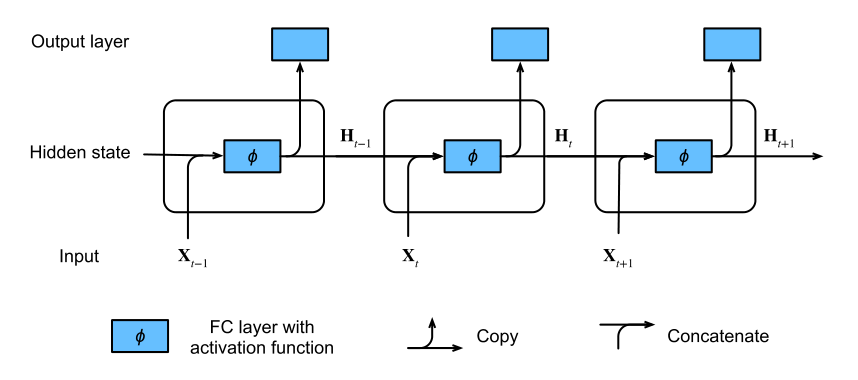
\includegraphics[width=0.8\linewidth]{images/rnn}
    \caption{Una RNN con un estado escondido.}
    \label{fig:rnn}
\end{figure}



\subsubsection{\textit{Gated Recurrent Units}}

Uno de los principales desafíos en la predicción de datos secuenciales es el de lograr preservar información de largo plazo al tiempo de ser capaces de ignorar entradas en el corto plazo que sean irrelevantes o que aporten poca información.

Estas consideraciones son de particular importancia cuando hallamos secuencias que tienen saltos estructurales que deseamos aprender. Por enunciar un ejemplo, consideremos lo que sucede cuando pasamos en un texto de un capítulo a otro. La ruptura lógica en el contexto de la secuencia es un factor que deseamos que nuestras redes neuronales sean capaces de capturar.

Uno de los primeros intentos para enfrentar este problema fue el diseño de las redes recurrentes conocidas como \textit{Long--Short Term Memory} (LSTM) \parencite{Hochreiter1997}. En esta sección describimos una arquitectura más moderna que pretende resolver esos mismos problemas, consiguiendo resultados comparables \parencite{Chung2014}.

Las \textit{Gated Recurrent Units} ---GRU por sus siglas en inglés--- son un tipo de RNN que toman aparente inspiración de las puertas lógicas de circuitos, al incorporar unidades escondidas que funcionan de manera aproximada a puertas, y que permiten a la red neuronal controlar cuánta información del estado actual $ \X_t $ se pasa al siguiente estado y cuánta del estado escondido anterior $ \hi_{t-1} $ se retiene.

Las primeras unidades que introducimos son la \textit{puerta de reinicio} y la \textit{puerta de actualización}. La puerta de reinicio le permite controlar a la red cuánta información del anterior estado deseamos preservar. A su vez, la puerta de actualización nos permite controlar en qué medida el nuevo estado es una copia del anterior.

En términos matemáticos, para un tiempo $ t $ dado y un minilote $ \X_t \in \R^{n\times d} $ ---con $ n $ ejemplos y $ d $ dimensiones por ejemplo-- y un estado escondido del anterior paso $ \hi_{t-1} \in \R^{n \times h} $ ---con $ h $ unidades escondidas---, la puertas de reinicio y actualización $ \res_t \in \R^{n \times h} $, $ \upd_t \in \R^{n \times h} $, respectivamente, están dadas por:
\begin{align}
    \res_t &= \sigma(\X_t \we_{xr} + \hi_{t-1}\we_{hr} + \bi_r), \\
    \upd_t &= \sigma(\X_t \we_{xz} + \hi_{t-1}\we_{hz} + \bi_z),
\end{align}
donde $ \we_{xr}, \we_{xz} \in \R^{d \times h} $ y $ \we_{hr}, \we_{hz} \in \R^{h \times h} $ son parámetros de pesos y $ \bi_r, \bi_z \in \R^{1 \times h} $ son vectores de sesgo. Refiérase a la \cref{fig:gru-1}.

Notemos que utilizamos funciones sigmoideas para la activación de estas unidades elemento a elemento, de modo que las salidas se encontrarán siempre en el intervalo $ (0,1) $.

\begin{figure}
    \centering
    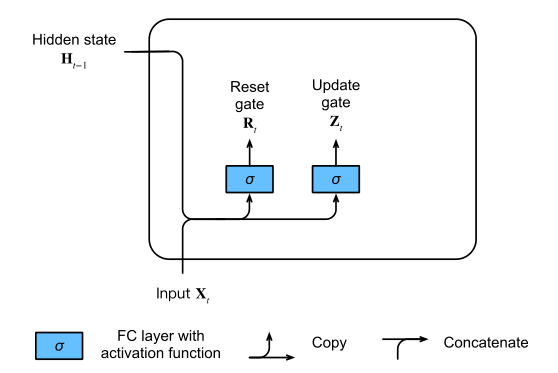
\includegraphics[width=0.7\linewidth]{images/gru-1}
    \caption{Cálculo de las puertas de reinicio y actualización en un modelo GRU.}
    \label{fig:gru-1}
\end{figure}

El siguiente paso consiste en integrar la información en la puerta de reinicio con la contenida en el estado escondido y la entrada del tiempo actual. En términos matemáticos, generamos un \textit{candidato a estado escondido} $ \tilde{\hi}_t \in \R^{n \times h} $ al tiempo $ t $, dado por:
\begin{equation}
    \tilde{\hi}_t = \tanh(\X_t \we_{xh} + (\res_t \odot \hi_{t-1})\we_{hh} + \bi_h),
\end{equation}
donde $ \we_{xh} \in \R^{d \times h} $ y $ \we_{hh} \in \R^{h \times h} $ son parámetros de pesos, $ \bi_h \in \R^{1 \times h} $ es el sesgo, y el símbolo $ \odot $ es el producto de Hadamard elemento a elemento entre dos matrices de las mismas dimensiones. Observemos primero que utilizamos la no--linealidad de $ \tanh $ para hacer que los valores del candidato a estado escondido permanezcan en el intervalo $ (-1, 1) $.

Notemos que si las entradas de la puerta de reinicio $ \res_t $ son todas 1, recuperamos la RNN que presentamos en la \cref{eq:rnn}. Análogamente, si todas las entradas de $ \res_t $ son 0, entonces el candidato a estado escondido contiene únicamente información de la entrada $ \X_t $. En otras palabras, cualquier estado escondido preexistente se \textit{reinicia}. Refiérase a la \cref{fig:gru-2}.

\begin{figure}
    \centering
    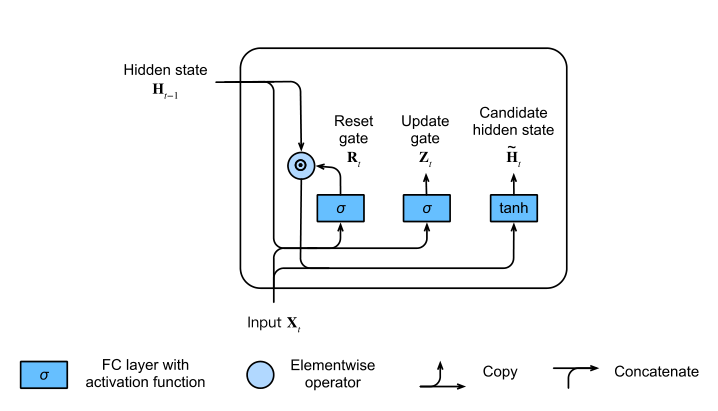
\includegraphics[width=0.8\linewidth]{images/gru-2}
    \caption{Cálculo del candidato a estado escondido en un modelo GRU.}
    \label{fig:gru-2}
\end{figure}


Finalmente, incorporamos el efecto de la puerta de actualización $ \upd_t $. Esta determina en qué medida el nuevo estado escondido $ \hi_t \in \R^{n\times h} $ contiene información del anterior estado $ \hi_{t-1} $, y en qué medida contiene información del candidato a estado escondido $ \tilde{\hi}_t $. Logramos ésto haciendo una combinación lineal convexa entre $ \hi_{t-1} $ y $ \tilde{\hi}_t $:
\begin{equation}
    \hi_t = \upd_t \odot \hi_{t-1} + (1 - \upd_t) \odot \tilde{\hi}_t.
\end{equation}
De manera análoga al anterior paso, observemos que si las entradas de la puerta de actualización son todas 1, entonces el estado escondido $ \hi_t $ contendrá información únicamente del anterior estado escondido $ \hi_{t-1} $, mientras que si son todas 0, el nuevo estado escondido contendrá únicamente información del candidato a estado escondido $ \tilde{\hi}_t $. Refiérase a la \cref{fig:gru-3}.

\begin{figure}
    \centering
    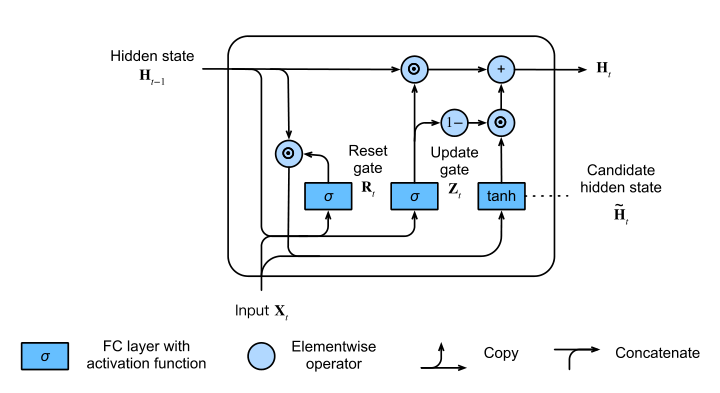
\includegraphics[width=0.8\linewidth]{images/gru-3}
    \caption{Cálculo del estado escondido en un modelo GRU.}
    \label{fig:gru-3}
\end{figure}

Estos diseños nos permiten capturar dependencias en secuencias muy largas. Por ejemplo, si la puerta de actualización ha sido cercana a 1 para todos los pasos de tiempo de alguna subsecuencia, el anterior estado escondido al tiempo de su inicio será mayormente retenido y pasado hasta el final de la subsecuencia, independientemente de la longitud de la subsecuencia.

En resumen, las GRUs tienen las siguientes características sobresalientes:
\begin{itemize}
    \item Las puertas de reinicio capturan dependencias de corto plazo en secuencias.
    \item Las puertas de actualización capturan dependencias de largo plazo en las secuencias.
\end{itemize}

\subsubsection{RNNs profundas}

El siguiente paso para flexibilizar las redes recurrentes que hemos descrito hasta ahora consiste en agregar más capas de RNNs para aumentar la capacidad de estas redes de capturar dinámicas no--lineales más complejas.

\begin{figure}
    \centering
    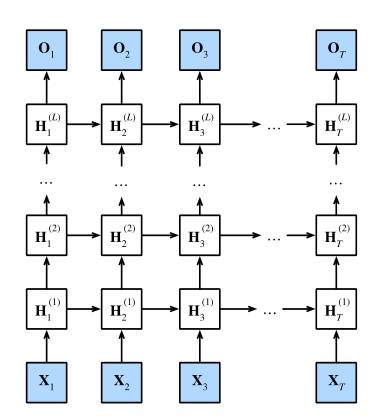
\includegraphics[width=0.5\linewidth]{images/deep-rnns}
    \caption{Arquitectura de una RNN profunda.}
    \label{fig:deep-rnns}
\end{figure}

Refiérase a la \cref{fig:deep-rnns} para una representación gráfica de la arquitectura que planteamos.

Matemáticamente, para un minilote de ejemplos $ \X_t \in \R^{n \times d} $ (con $ n $ ejemplos y $ d $ dimensiones de entrada) al tiempo $ t $, denominamos a la $ l $--ésima capa escondida $ \hi_t^{(l)} \in \R^{n \times h} $ (con $ h $ unidades escondidas) para $ l \in \{1, 2, \ldots, L\} $, donde $ \hi_t^{(0)} = \X_t $. A su vez, denominamos a la variable de la capa de salida $ \out_t \in \R^{n \times q} $ (con $ q $ unidades de salida). Así, el estado escondido de la $ l $--ésima capa de salida que usa la función de activación $ \phi_t $ está dado por:
\begin{equation}
    \hi_t^{(l)} = \phi_t(\hi_t^{(l-1)}\we_{xh}^{(l)} + \hi_{t-1}^{(l)}\we_{hh}^{(l)} + \bi_h^{(l)}),
\end{equation}
donde los pesos $ \we_{xh}^{(l)} \in \R^{d\times h} $ y $ \we_{hh}^{(l)} \in \R^{h \times h} $ junto con el vector de sesgo $ \bi_h^{(l)} \in \R^{1 \times h} $ constituyen los parámetros de de la \textit{l}--ésima capa escondida.

Después del cálculo de todas las capas escondidas, el cálculo de la capa de salida utiliza únicamente la información contenida en la $ L $--ésima capa escondida. Es decir:
\begin{equation}
    \out_t = \hi_t^{(L)}\we_{hq} + \bi_q,
\end{equation}
donde $ \we_{hq} \in \R^{h \times q} $ son los parámetros de pesos respectivos y el sesgo es $ \bi_q \in \R^{1 \times q} $.

\subsubsection{RNNs bidireccionales}

Como mencionamos antes, las RNNs que hemos descrito hasta ahora son \textit{unidireccionales}, en el sentido de que la información fluye conforme avanza el tiempo $ t $.

En aprendizaje de secuencias existen tareas para las que la salida de una predicción puede depender de \textit{toda la secuencia de entrada}. Por ejemplo, en reconocimiento de voz, la correcta interpretación de un sonido como un fonema puede depender de los siguientes sonidos por un fenómeno conocido como co--articulación. Si hay varias interpretaciones de una palabra y ambas son acústicamente plausibles, probablemente necesitaremos obtener información del pasado y del futuro de la sucesión para desambiguarlas. 

Este mismo fenómeno se presenta en reconocimiento de escritura a mano, en análisis de sentimientos (que en el fondo es una tarea de clasificación de secuencias), en traducción automática de textos, y en otras tareas de aprendizaje de secuencia a secuencia.

Las RNNs bidireccionales se inventaron para resolver este tipo de problemas \parencite{Schuster1997}. Para obtener información de toda la secuencia, utilizaremos una RNN que pase información en la dirección del tiempo de la secuencia, y la acoplaremos a otra que pase información en la dirección contraria. La \cref{fig:bidirectional-rnns} muestra la arquitectura de una RNN bidireccional con una sola capa escondida.

\begin{figure}
    \centering
    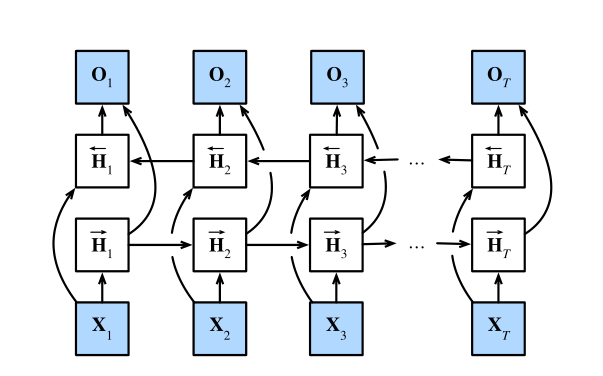
\includegraphics[width=0.7\linewidth]{images/bidirectional-rnns}
    \caption{Arquitectura de una RNN bidireccional.}
    \label{fig:bidirectional-rnns}
\end{figure}

Matemáticamente, para un minilote de ejemplos $ \X_t \in \R^{n \times d} $ (con $ n $ ejemplos y $ d $ dimensiones de entrada) al tiempo $ t $, denominamos por $ \overrightarrow{\hi}_t \in \R^{n \times h} $ al estado escondido que pasa información en la dirección del tiempo. Análogamente, denominamos por $ \overleftarrow{\hi}_t \in \R^{n \times h} $ al estado escondido que pasa información en la dirección contraria al tiempo, y nombramos a estos estados escondidos \textit{estado escondido hacia adelante} y \textit{estado escondido hacia atrás}, respectivamente. El cálculo de estos está dado por:
\begin{align}
    \overrightarrow{\hi}_t &= \phi(\X_t\we_{xh}^{(f)} + \overrightarrow{\hi}_{t-1}\we_{hh}^{(f)} + \bi_h^{(f)}), \\
    \overleftarrow{\hi}_t &= \phi(\X_t\we_{xh}^{(b)} + \overleftarrow{\hi}_{t-1}\we_{hh}^{(b)} + \bi_h^{(b)}),
\end{align}
donde los pesos $ \we_{xh}^{(f)}, \we_{xh}^{(b)} \in \R^{d \times h} $, $ \we_{hh}^{(f)}, \we_{hh}^{(b)} \in \R^{h \times h} $ $ \bi_h^{(l)} \in \R^{1 \times h} $ y los sesgos $ \bi_h^{(f)}, \bi_h^{(b)} \in \R^{1 \times h} $ son todos los parámetros del modelo.

Después de hacer el cálculo de los estados escondidos hacia adelante y hacia atrás $ \overrightarrow{\hi}_t $ y $ \overleftarrow{\hi}_t $, concatenamos estos estados para obtener el estado $ \hi_t \in \R^{n \times 2h} $ que pasamos a la capa de salida. En RNNs bidireccionales con varias capas, esta información la pasamos como entrada a la siguiente capa bidireccional. 

Para computar la salida de la red neuronal tenemos $ \out_t \in \R^{n \times q} $ (con $ q $ salidas):
\begin{equation}
    \out_t = \hi_t^{(l)}\we_{hq} + \bi_q,
\end{equation}
donde $ \we_{hq} \in \R^{2h \times q} $ son los parámetros de pesos respectivos y el sesgo es $ \bi_q \in \R^{1 \times q} $ para la \textit{l}--ésima capa, con $l \in \{1, 2, \ldots, L\}$.

Es importante mencionar que el costo computacional de entrenar una RNN bidireccional es muy elevado, dado que la fase de propagación hacia adelante requiere hacer cálculos recursivos hacia adelante y hacia atrás en las capas bidireccionales, y que la retropropagación depende a su vez de las salidas de la propagación hacia adelante. Así, los gradientes tienen largas cadenas de dependencias.

\subsubsection{Arquitecturas \textit{encoder}--\textit{decoder}}

El último componente que introducimos es el de la arquitectura \textit{encoder}--\textit{decoder}, que es una de las arquitecturas idóneas para hacer aprendizaje de secuencia a secuencia. 

Las arquitecturas \textit{encoder}--\textit{decoder} tienen dos grandes componentes: un codificador (\textit{encoder}) y un decodificador (\textit{decoder}). El diseño de estas redes puede observarse en la \cref{fig:encoder-decoder}.

\begin{figure}
    \centering
    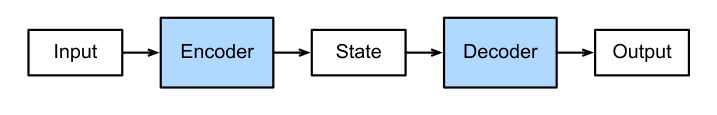
\includegraphics[width=0.7\linewidth]{images/encoder-decoder}
    \caption{Arquitectura \textit{encoder}--\textit{decoder}.}
    \label{fig:encoder-decoder}
\end{figure}

El codificador convierte las secuencias de entrada en una representación de un espacio latente; esta información se pasa como entrada al decodificador, que se encarga de convertir la representación obtenida en la salida que se requiera. Puede ser otra secuencia, una clasificación, el predictor continuo de una regresión, etc. Desde luego, en la elección de la arquitectura del decodificador debe tomarse en cuenta el tipo de salida.

\subsection{\textit{Word embeddings}}

Cuando se realizan tareas de aprendizaje de secuencias debemos abordar necesariamente el problema de cómo representar estas secuencias como entradas de una red. En tareas de procesamiento de lenguaje natural como la que abordamos, comenzamos siempre por generar un mapeo biyectivo entre todos los tokens únicos ---palabras, letras, símbolos, fonemas, etc.---  del corpus e índices que los identifiquen únicamente. 

Si bien la representación numérica de tokens es mucho más eficiente en términos de memoria que si guardásemos los \textit{strings} y los usáramos como entradas directamente a una red neuronal de alguna manera, una representación basada únicamente en números es posiblemente una mala representación de los tokens. 

La forma más simple de representar los tokens es utilizando \textit{one--hot encoding}. En esta representación codificamos cada token como un vector con tantas entradas como tokens únicos tiene el vocabulario del corpus cuyas entradas son todas 0 salvo por la entrada correspondiente al índice del token, que es 1. Es decir, que el \textit{one--hot encoding} del $ i $--ésimo token es el vector $ (x_1, x_2, ..., x_d) $, donde $ x_j = 1 $ si $ j = i $ y $ x_j = 0 $ si $ j \neq i $.

Si bien esta representación facilita ciertos cálculos, como el cálculo de pérdida durante la fase de entrenamiento, la representación es altamente dispersa, y los vectores suelen ser de dimensión muy alta. Notemos además que al formar un conjunto ortogonal, somos incapaces de utilizar medidas de similitud para determinar si dos tokens comparados son similares o no. 

Las técnicas que presentamos en esta sección tienen por objetivo hallar representaciones eficientes y dotadas de estructura que puede ayudar para mejorar el desempeño del modelo neuronal que construyamos.

\subsubsection{\code{word2vec} (\textit{skip--gram})}

La herramienta \code{word2vec} fue propuesta para abordar los anteriores problemas \parencite{Mikolov2013}. El modelo mapea cada palabra en el vocabulario dado a un vector de longitud fija, y estos vectores pueden expresar mejor las relaciones de analogía y similitud entre diferentes palabras. La herramienta contiene dos modelos: \textit{skip--gram} y \textit{continuous bag of words} (CBOW), de los cuales nosotros describimos únicamente el primero.

El modelo \textit{skip--gram} asume que una palabra se puede utilizar para generar sus palabras aledañas en una secuencia de texto. Tomemos la secuencia de texto "<el">, "<hombre">, "<ama">, "<viajar">, "<mucho"> como ejemplo, elijamos la palabra "<ama"> como \textit{palabra central} y una \textit{ventana de contexto} igual a 2. 

Dada la palabra central "<ama">, el modelo \textit{skip--gram} considera la probabilidad condicional de las \textit{palabras contextuales}: "<el">, "<hombre">, "<viajar">, "<mucho"> que están a no más de 2 palabras de la palabra central:
\begin{equation}
    P(\text{"<el">, "<hombre">, "<viajar">, "<mucho">}\mid\text{"<ama">}). \label{eq:skip1}
\end{equation}

Si asumimos que las palabras contextuales son generadas independientemente dada la palabra central (en el sentido de independencia condicional), entonces la \cref{eq:skip1} puede reescribirse como:
\begin{equation}
    P(\text{"<el">}\mid\text{"<ama">}) \cdot P(\text{"<hombre">}\mid\text{"<ama">}) \cdot P(\text{"<viajar">}\mid\text{"<ama">}) \cdot P(\text{ "<mucho">}\mid\text{"<ama">}).
\end{equation}

En el modelo \textit{skip--gram} cada palabra tiene 2 vectores $ d $--dimensionales para calcular las probabilidades condicionales. Concretamente, para alguna palabra con índice $ i $ en el vocabulario, denotamos por $ \ce_i \in \R^{d} $ y $ \co_i \in \R^{d} $ sus dos vectores: cuando es usada como palabra central, y cuando es usada como palabra de contexto, respectivamente. 

La probabilidad condicional de generar cualquier palabra contextual $ w_o $ (con índice $ o $ en el vocabulario) dada la palabra central $ w_c $ (con índice $ c $ en el diccionario) puede modelarse con una operación \textit{softmax} sobre productos punto como sigue:
\begin{equation}
    P(w_o \mid w_c) = \frac{\exp(\co_o^{\top}\ce_c)}{\sum_{i \in \mathcal{V}}\exp(\co_i^{\top}\ce_c)},
\end{equation}
donde el conjunto de índices del vocabulario es $ \mathcal{V} = \{0, 1, \ldots, |\mathcal{V}| - 1\} $.


Para entrenar el modelo \textit{skip--gram} utilizamos el método de máxima verosimilitud. Para ello recordemos que la función de verosimilitud es la probabilidad conjunta de observar los datos obtenidos como función de los parámetros del modelo. 

En este caso, los parámetros son los vectores de palabra central y de palabra contextual de cada palabra en el vocabulario. La función de verosimilitud del modelo es, así, la probabilidad de generar todas las palabras contextuales dada cualquier palabra central como función de los vectores de palabra central y de palabra contextual de cada palabra en el vocabulario.

Matemáticamente, dada una secuencia de texto de largo $ T $, donde la palabra al tiempo $ t $ se denota por $ w^{(t)} $, si asumimos que las palabras contextuales son condicionalmente independientes de cualquier palabra central, entonces para una ventana de contexto $ m $, la función de verosimilitud de \textit{skip--gram} está dada por:
\begin{equation}
    \prod_{t=1}^{T} \prod_{\substack{-m \leq j \leq m, \\ j\neq 0}} P(w^{(t+j)} \mid w^{(t)}),
\end{equation}
donde cualquier tiempo menor que 1 o mayor que $ T $ es ignorado.

Observemos que maximizar la anterior función de verosimilitud es equivalente a minimizar la siguiente función de pérdida:
\begin{equation}
    -\sum_{t=1}^{T} \sum_{\substack{-m \leq j \leq m, \\ j\neq 0}} \log P(w^{(t+j)} \mid w^{(t)}), \label{eq:skip-gram loss}
\end{equation}
donde:
\begin{equation}
    \log P(w^{(t+j)} \mid w^{(t)}) = \co_o^{\top}\ce_c - \log\left(\sum_{i \in \mathcal{V}}\exp(\co_i^{\top}\ce_c) \right).
\end{equation}

Para obtener los gradientes de la anterior función de pérdida respecto de los parámetros del modelo, diferenciamos normalmente. Como ejemplo, el gradiente respecto del vector $ \ce_c $ está dado por:
\begin{align}
    \frac{\partial \log P(w^{(t+j)} \mid w^{(t)})}{\partial \ce_c} &= \co_o - \frac{\sum_{j \in \mathcal{V}}\exp(\co_j^{\top}\ce_c)\co_j}{\sum_{i \in \mathcal{V}}\exp(\co_i^{\top}\ce_c)} \\
    &= \co_o - \sum_{j \in \mathcal{V}} \left( \frac{\exp(\co_j^{\top}\ce_c)}{\sum_{i \in \mathcal{V}}\exp(\co_i^{\top}\ce_c)} \right)\co_j \\
    &= \co_o - \sum_{j \in \mathcal{V}} P(w_j \mid w_c)\co_j.
\end{align}

Los gradientes para los otros vectores de palabras pueden obtenerse de modo similar.

Por último, en una nota técnica, notemos que como no utilizamos datos anotados en este proceso de aprendizaje, este algoritmo se conoce como de aprendizaje auto--supervisado.

El resultado del entrenamiento de este modelo ---los vectores de palabra central y de contexto de todas las palabras--- puede ser incorporado a un modelo de redes neuronales con una capa de \textit{embedding} que realiza una búsqueda y devuelve las representaciones vectoriales obtenidas para los tokens que componen las secuencias de nuestro corpus. Dichos vectores pueden ser pasados como entrada a otras unidades de una red neuronal ---como por ejemplo, a una unidad \textit{encoder}---.

\subsubsection{\textit{GloVe}}

\textit{Global Vectors} \parencite{Pennington2014} es un modelo de \textit{word embeddings} que ha tenido muy buenos resultados en tareas de aprendizaje de secuencias y que trata de resolver algunos problemas computacionales presentes en \code{word2vec}. Para entender mejor estos problemas revisitemos el modelo \textit{skip--gram} para introducir notación esencial.

Primero denotemos por $ q_{ij} $ a la probabilidad condicional de tener la palabra contextual $ w_j $ dada la palabra central $ w_i $ en el modelo \textit{skip--gram}; esto es:
\begin{equation}
    q_{ij} = \frac{\exp(\co_j^{\top}\ce_i)}{\sum_{k \in \mathcal{V} \exp(\co_{k}^{\top}\ce_i)}},
\end{equation}
donde para cualquier índice $ i $, $ \ce_i $ y $ \co_i $ son los vectores de la palabra $ w_i $ como palabra central y contextual, respectivamente, y $ \mathcal{V} = \{0, 1, \ldots, |\mathcal{V}| - 1\} $ es el conjunto de índices en el vocabulario.

Consideremos una palabra $ w_i $ que puede aparecer varias veces en el corpus. Denotemos por $ \mathcal{C}_i $ al multiconjunto ---es decir, que sus elementos pueden estar contenidos varias veces--- de los índices de todas las palabras contextuales en el corpus que tienen a $ w_i $ como palabra central dada una ventana de contexto fija. 

Al número de veces que ocurre la palabra con índice $ j $ en el multiconjunto $ \mathcal{C}_i $ lo denotamos por $ x_{ij} $. Utilizando esta estadística global del corpus, la función de pérdida del modelo \textit{skip--gram} ---\cref{eq:skip-gram loss}--- puede escribirse como:
\begin{equation}
    -\sum_{i \in \mathcal{V}}\sum_{j \in \mathcal{V}} x_{ij} \log q_{ij}. \label{eq:skip-gram again}
\end{equation}

Ahora, si denotamos por $ x_i $ al conteo de todas las palabras contextuales que tienen a $ w_i $ como palabra central ---es decir, $ x_i = |\mathcal{C}_i| $---, y si denotamos por $ p_{ij} $ al estimador de la probabilidad condicional de obtener la palabra contextual $ w_j $ dada la palabra central $ w_i $ ---es decir, $ p_{ij} =  x_{ij}/x_i $, la \cref{eq:skip-gram again} puede reescribirse como:
\begin{equation}
    -\sum_{i \in \mathcal{V}} x_{i}\sum_{j \in \mathcal{V}} p_{ij} \log q_{ij}.
\end{equation}

En la anterior expresión, observemos que el término $ -\sum_{j \in \mathcal{V}} p_{ij} \log q_{ij} $ calcula la entropía cruzada de la distribución condicional de las estadísticas globales del corpus $ p_{ij} $ y la distribución condicional $ q_{ij} $ de predicciones del modelo. Desde este punto de vista es fácil ver que la función de pérdida en la \cref{eq:skip-gram loss} es una suma ponderada de la entropía cruzada entre las distribuciones $ p_{ij} $ y $ q_{ij} $.

% TODO: referencias
Los autores de GloVe argumentan que utilizar las co--ocurrencias de palabra a palabra, que definimos como $ p_{ik}/p_{jk} $, en lugar de las probabilidades condicionales por sí solas, nos guía a una representación vectorial que aprovecha mejor estas estadísticas globales. Esta representación es el modelo GloVe, que además resuelve el problema de que normalizar apropiadamente $ q_{ij} $ resulta en la suma sobre todo el vocabulario, que puede ser computacionalmente muy costoso, y además no sufre del problema de que el modelado por entropía cruzada lleva, en corpus grandes, a que co--ocurrencias raras tengan demasiado peso.

Los autores de GloVe realizan tres cambios al modelo \textit{skip--gram} utilizando un modelo de regresión log--cuadrática:
\begin{enumerate}
    \item Usamos las variables $ p'_{ij} = x_{ij} $ y $ q'_{ij} = \exp(\co_j^{\top}\ce_{i}) $ que no son distribuciones de probabilidad, y toman el logaritmo de ambas, así que el término de pérdida cuadrático es $ \left( \log p'_{ij} - \log q'_{ij}\right)^2 = \left( \co_j^{\top}\ce_i - \log x_{ij} \right)^2 $.
    
    \item Agregan dos parámetros escalares al modelo para cada palabra $ w_i $: el sesgo de palabra central $ b_i $ y el sesgo de palabra contextual $ c_i $.
    
    \item Remplazan el peso de cada término en la función de pérdida con la función de peso $ h(x_{ij}) $, donde $ h $ es creciente en el intervalo $ [0,1] $. Una forma que puede adquirir esta función es $ h(x) = (x / c)^{\alpha} $ si $ x < c $, y $ h(x) = 1 $ en otro caso, para alguna $ \alpha > 0 $.
\end{enumerate}

La función de pérdida resultante del modelo GloVe está dada por:
\begin{equation}
    \sum_{i \in \mathcal{V}}\sum_{j \in \mathcal{V}}h(x_{ij}) \left( \co_j^{\top}\ce_i + b_i + c_i - \log x_{ij} \right)^2.
\end{equation}

Una vez que los vectores contextuales y centrales de todas las palabras han sido determinados a través del proceso de entrenamiento por descenso estocástico de gradiente, los vectores resultantes se suman para obtener la representación final.

\section{Arquitectura final}

La arquitectura final que utilizamos en este proyecto utiliza todos los elementos que hemos incluido en el marco teórico. 

Recordemos que la tarea que intentamos resolver en este proyecto es la clasificación de sentimiento de tuits en español de México, utilizando redes neuronales recurrentes y \textit{word embeddings}. Para una referencia de la arquitectura final observe la \cref{fig:final}.

\begin{figure}
    \centering
    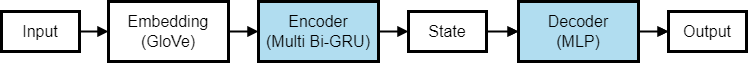
\includegraphics[width=0.9\linewidth]{images/final}
    \caption{Arquitectura final para clasificación de sentimiento.}
    \label{fig:final}
\end{figure}

Utilizamos vectores pre--entrenados en español siguiendo el modelo GloVe, y usamos dichas representaciones utilizando una capa de \textit{embedding} que pasa las representaciones vectoriales de las secuencias de entrada al \textit{encoder}. 

El \textit{encoder} es una red GRU bidireccional de varias capas que sirve para codificar la información de cada tuit (en tanto que una sucesión completa de tokens) en un espacio latente que se pasa como entrada al \textit{decoder}.

Finalmente, el \textit{decoder} es una red de perceptrón multicapa completamente conectada. Esta red tendrá como objetivo traducir las representaciones de las secuencias en el estado latente a una representación vectorial de \textit{one--hot encoding} de las tres categorías de interés: "<positivo">, "<negativo"> y "<neutro">. La función de pérdida que utilizamos es de entropía cruzada.


\printbibliography[title={Referencias y bibliografía}]

\end{document}
